\documentclass{article}
\usepackage[utf8]{inputenc}
% -------------------- Packages --------------------
\usepackage{amsmath}
\usepackage{amssymb}
\usepackage[noend]{algpseudocode}
\usepackage{algorithm}
\usepackage{graphicx}
\usepackage{float}
\usepackage{fontawesome5}
\usepackage{listings}

\lstset{language=Python,keywordstyle={\bfseries \color{blue}}}
\NewDocumentCommand{\codeword}{v}{%
    \texttt{\textcolor[HTML]{5c5c65}{#1}}%
}


\usepackage{hyperref}
\hypersetup{
    colorlinks=true,
    linkcolor=blue,
    filecolor=magenta,      
    urlcolor=cyan,
    pdftitle={Overleaf Example},
    pdfpagemode=FullScreen,
    }

\urlstyle{same}

\usepackage{bookmark}
\hypersetup{hidelinks} %enlève les cadres rouges autour des hyperliens


% ---------- PSEUDO CODE : hack to remove indent ----------
% https://tex.stackexchange.com/questions/354564/how-to-remove-leading-indentation-from-algorithm
\usepackage{xpatch}
\makeatletter
\xpatchcmd{\algorithmic}
  {\ALG@tlm\z@}{\leftmargin\z@\ALG@tlm\z@}
  {}{}
\makeatother

\usepackage{xcolor}
\usepackage[framemethod=tikz]{mdframed}
\usepackage{tikzpagenodes}
\usetikzlibrary{calc}


% add foreach
\algnewcommand\algorithmicforeach{\textbf{for each}}
\algdef{S}[FOR]{ForEach}[1]{\algorithmicforeach\ #1\ \algorithmicdo}


% -------------------- Couleurs --------------------
\definecolor{definition}{HTML}{2f80ed}
\definecolor{definition-bg}{HTML}{e0ecfd}

\definecolor{danger-color}{HTML}{e6505f}
\definecolor{danger-bg-color}{HTML}{fce5e7}

\definecolor{gris-color}{HTML}{dadce0}
\definecolor{blanc-color}{HTML}{fcfcfc}

\definecolor{underbrace-color}{HTML}{a0a0a0}

% -------------------- Code --------------------
\definecolor{codegreen}{rgb}{0,0.6,0}
\definecolor{codegray}{rgb}{0.5,0.5,0.5}
\definecolor{codepurple}{rgb}{0.58,0,0.82}
\definecolor{backcolour}{rgb}{0.95,0.95,0.92}

\lstdefinestyle{code-style}{
    backgroundcolor=\color{backcolour},   
    commentstyle=\color{codegreen},
    keywordstyle=\color{magenta},
    numberstyle=\tiny\color{codegray},
    stringstyle=\color{codepurple},
    basicstyle=\ttfamily\footnotesize,
    breakatwhitespace=false,         
    breaklines=true,                 
    captionpos=b,                    
    keepspaces=true,                 
    numbers=left,                    
    numbersep=5pt,
    showspaces=false,                
    showstringspaces=false,
    showtabs=false,                  
    tabsize=2
}


% -------------------- Macros --------------------
\mdfdefinestyle{definition-style}{%
  innertopmargin=10px,
  innerbottommargin=10px,
  linecolor=definition,
  backgroundcolor=definition-bg,
  roundcorner=4px
}
\newmdenv[style=definition-style]{definition}

\newcommand\testos[1]{clovis{\MakeUppercase #1}}

\newcommand\clovisColorfulBlock[1]{
    % #1 = danger (name)
    % #2 = danger-color (color)
    % #3 = danger-bg-color (background color)
    \mdfdefinestyle{#1-style}{%
        innertopmargin=10px,
        innerbottommargin=10px,
        linecolor=#1-color,
        backgroundcolor=#1-bg-color,
        roundcorner=4px
    }
    \newmdenv[style=#1-style]{#1}

    
    \expandafter\newcommand\csname clovis#1\endcsname[1]{
        \begin{#1}
        {\scriptsize \textcolor{#1-color}{\faIcon{exclamation-triangle} \textbf{DANGER}}}
        \vspace{3px}
        \\ ##1
        \end{#1}
    }
}

\clovisColorfulBlock{danger}

\newcommand\clovisDefinition[2]{
    \begin{definition}
    { \scriptsize \textcolor{definition}{\faIcon{graduation-cap} \textbf{DEFINITION}}}
    \vspace{3px}
    \\ \underline{\textbf{#1}}
    \vspace{2.5px}
    \\ #2
    \end{definition}
}


\newcommand\underbraceColor[2]{
    \color{underbrace-color} % set color to grey
    
    \underbrace{
        \color{black}{#1} % set color back to black
    }_{
        \text{#2}
    }
    
    \color{black} % set color back to black
}



% -------------------- Test color box --------------------
\usepackage[most]{tcolorbox}
\tcbset{on line, 
        boxsep=3px, left=0pt,right=0pt,top=0pt,bottom=0pt,
        boxrule=0.5px,
        colframe=gris-color,colback=blanc-color,  
        highlight math style={enhanced}
        }

% -------------------- Document --------------------
\title{Optimisation dans les Réseaux}
\author{}
\date{Licence 3\\2021 - 2022}
\begin{document}
\normalsize
\maketitle

\renewcommand*\contentsname{Table des matières}
\tableofcontents
\newpage
\section{Introduction}

\begin{figure}[H]
    \centering
    \scalebox{0.5}{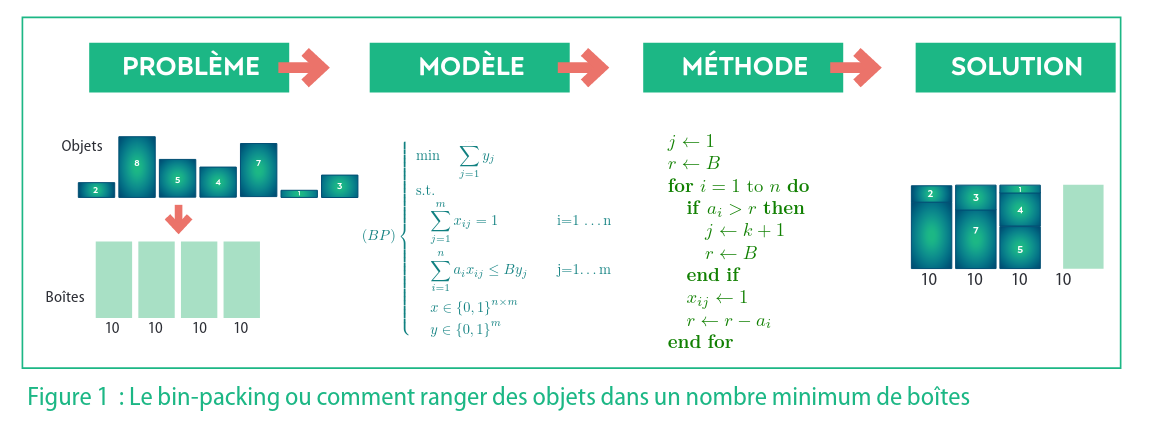
\includegraphics{img/bin-packing.png}}
\end{figure}

$a_i$ = taille de l'objet i
\\\\%
$y_i \begin{cases}
   0 & \text{si la boite n'est pas utilisée} \\
   1 & \text{si la boite est utilisée}
\end{cases}
\\\\x_{i, j} \begin{cases}
   0 & \text{si l'objet i n'est pas dans la boîte j} \\
   1 & \text{si l'objet i est dans la boîte j}
\end{cases}
$
\\\\%
$x_{1, 1} + x_{1, 2} + ... + x_{1, 7} = 1$ $\rightarrow$ cela veut dire que l'objet 1 est dans \textbf{une} seule boîte
\\\\%
On cherche à minimiser le nombre de boîtes, donc :
$$\min \sum_{j=1}^{7} y_j$$
%
\clovisDefinition{Adjacence}{
   Entre deux éléments de même nature.
}

\clovisDefinition{Incidence}{
    Entre deux éléments de nature différente.
}

\begin{figure}[H]
    \centering
    \scalebox{1}{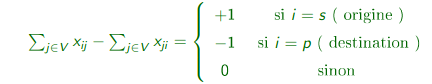
\includegraphics{img/eq_chemin.png}}
    $$
    \sum_{j \in V} \underbraceColor{x_{i, j}}{degré sortant} - \sum_{j \in V} x_{j, i} =  \begin{cases}
       +1 & \text{si } i = s \text{ (origine)}\\
       -1 & \text{si } i = p \text{ (destination)} \\
       0 & \text{sinon}
    \end{cases}
    $$
    Cette équation signifie : par un noeud passe \textbf{un seul} chemin.
    \\A gauche degré sortant, à droite degré entrant.
\end{figure}
Il y a un arc entrant ($-1$) et un arc sortant (+1) : on obtient donc 0, sauf si c'est l'origine (arc \textbf{sortant} uniquement, donc 1) ou la destination (arc \textbf{entrant} uniquement, donc -1).
\begin{figure}[H]
    \centering
    \scalebox{0.5}{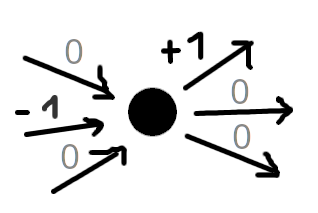
\includegraphics{img/chemins.png}}
\end{figure}








\end{document}

\clovisDefinition{Comment installer \tcbox{{\small\tt npm}}}{
    On utilise la commande \tcbox{{\small\tt npm install puppeteer}} pour installer \tcbox{{\small\tt puppeteer}} avec la console.
}

\clovisDefinition{Comment installer puppeteer}{
    On utilise la commande \tcbox{{\small\tt npm install puppeteer}} pour installer \tcbox{{\small\tt puppeteer}} avec la console.
}
%
Encadrer dans les maths : $a^2 + b^2 = \tcbhighmath{c^2}$
\\Tapez la commande \tcbox{{\small\tt print("Hello world")}} dans votre console.
%\\\fcolorbox{gris-color}{white}{\tt Salut}
%
Test longue ligne : \tcbox{{\small\tt print("Hello world"); print("Hello world"); print("Hello world"); print("Hello world"); print("Hello world"); print("Hello world"); }}
